\documentclass[12.1pt,a4paper]{article}

\usepackage{float}
\usepackage{fontspec}
\setmainfont{TeX Gyre Termes}

\usepackage{xcolor}
\definecolor{eqteal}{RGB}{14,124,107}

\usepackage{amsmath, amsfonts, amssymb}
\usepackage{unicode-math}
\setmathfont{TeX Gyre Termes Math}

\usepackage{geometry}
\geometry{top=1in, bottom=1in, left=1.1in, right=1.1in}

\usepackage{setspace}
\usepackage{microtype}
\usepackage{booktabs}
\usepackage{array}
\usepackage{placeins}
\usepackage{graphicx}
\graphicspath{{./}{docs/assets/}}

\usepackage{caption}
\captionsetup{
  font=small,
  labelfont=bf,
  justification=justified,
  singlelinecheck=false,
  skip=4pt
}

\usepackage{enumitem}
\usepackage{fancyhdr}
\usepackage{titlesec}
\usepackage{tikz}
\usetikzlibrary{arrows.meta, positioning}

% Links are blue on purpose: loaded once, no hidelinks override.
\usepackage[colorlinks=true, linkcolor=blue!70!black, urlcolor=blue!70!black, citecolor=blue!70!black]{hyperref}

\pagestyle{fancy}
\fancyhf{}
\lhead{\small Md.\ Ali Arman Rafi}
\rhead{\small Fairness-Constrained Educational Support}
\rfoot{\small\thepage}
\renewcommand{\headrulewidth}{0.45pt}
\renewcommand{\footrulewidth}{0pt}

\titleformat{\section}
  {\large\bfseries}
  {\thesection.}
  {0.55em}
  {}
\titleformat{\subsection}
  {\normalsize\bfseries}
  {\thesubsection.}
  {0.55em}
  {}
\titlespacing*{\section}{0pt}{10pt}{4pt}
\titlespacing*{\subsection}{0pt}{7pt}{2pt}

\setstretch{1.18}
\setlength{\parindent}{0pt}
\setlength{\parskip}{4pt}

\begin{document}

\begin{center}
\vspace*{2pt}

{\LARGE\bfseries\setstretch{1.2}
Fairness-Constrained Allocation of Educational Support in Rural Chattogram:\\[4pt]
Pricing the Trade-off Between Predictive Reach and Demographic Coverage}

\vspace{12pt}

{\large\bfseries Md.\ Ali Arman Rafi}\\[4pt]

{\normalsize
Department of Mathematics, University of Chittagong\\[3pt]
\href{mailto:sbrafi10@gmail.com}{Email}
\enspace\textbullet\enspace
\href{https://github.com/rafi-math}{GitHub}\\[5pt]
{\small\today}}
\end{center}

\vspace{6pt}

\begin{center}
\small
\href{https://github.com/rafi-math/edu-support-optimization-bd}{Repository}
\enspace\textbullet\enspace
\href{https://rafi-math.github.io/edu-support-optimization-bd/}{Project site}
\enspace\textbullet\enspace
\href{https://rafi-math.github.io/edu-support-optimization-bd/equireach.html}{Live dashboard}
\enspace\textbullet\enspace
\href{https://colab.research.google.com/github/rafi-math/edu-support-optimization-bd/blob/main/docs/phase3_reproduce_demo.ipynb}{Colab demo}
\end{center}

\vspace{4pt}

\noindent
\begin{minipage}{\textwidth}
\small\setstretch{1.3}
\textbf{Abstract: }\enspace
Support for out-of-school children is limited, so the real question is not only who is at risk, but who should be reached first. I estimate out-of-school risk for 4,861 children aged 6--17 in rural Chattogram from Bangladesh MICS 2019 microdata, then solve a budgeted selection problem with 730 packages. Ranking purely by predicted risk captures 332 of the 641 observed out-of-school children, yet selects only one child under 13. Adding coverage floors shows that age inclusion is expensive and gender inclusion is comparatively cheap, and the two floors are subadditive: at the proportional/parity corner the combined objective drop sits 5.74 units below the sum of the separate drops. The same selection step is published as a small dashboard that runs on fictional data or prepares a local run from a user's own file.
\end{minipage}

\vspace{4pt}
\noindent{\small\textit{Keywords:} operations research, educational targeting, mixed-integer programming, algorithmic fairness, survey microdata.}

% ── 1. Introduction ───────────────────────────────────────────
\section{Introduction}

A programme with a fixed number of support packages has to choose who gets them. A predictive model makes that choice easy to automate: rank children by estimated out-of-school risk and hand the packages to the top of the list. The trouble is what the top of the list looks like. In this cohort, out-of-school risk climbs steeply with age, so a pure risk ranking fills the budget with adolescents and leaves almost no room for younger children, even when those younger children are in genuine structural difficulty.

This report prices that trade-off rather than just asserting it. I build an out-of-fold risk score on verified MICS 2019 microdata for rural Chattogram, formulate the allocation as a budget-constrained mixed-integer program, and then impose lower-bound coverage floors for children under 13 and for girls, measuring what each floor costs in reach. The headline finding is that the two floors do not add up independently: imposing both is cheaper than the sum of their separate costs (interaction $-5.74$ at the proportional corner). I also ship the selection step as a working dashboard, so the method is not only described but usable.

% ── 2. Data, audit and the question ───────────────────────────
\section{Data, Audit and the Question}

The source is the children's file, \texttt{fs.sav}, of the Bangladesh Multiple Indicator Cluster Survey 2019~\cite{mics2019}. I keep rural households in Chattogram Division, children aged 6--17, with a valid school-attendance response. The raw rural cohort is 4,891 children. Thirty are dropped for incomplete interviews, zero survey weight, or missing core covariates, leaving a modeling-ready sample of $N = 4{,}861$. The target is out-of-school status in the current school year: 641 children, an unweighted rate of 13.19\% and a provisional child-weighted rate of 14.52\%. The support budget is $K = 730$, about 15\% of the sample. Table~\ref{tab:anchors} collects the anchors every later number is checked against.

\begin{table}[H]
\centering
\renewcommand{\arraystretch}{1.25}
\small
\begin{tabular}{@{}lr@{}}
\toprule
\textbf{Item} & \textbf{Value} \\
\midrule
Raw rural cohort & 4,891 children \\
Modeling-ready sample & 4,861 children \\
Observed out-of-school children & 641 \\
Unweighted out-of-school rate & 13.19\% \\
Provisional child-weighted rate & 14.52\% \\
Selection budget $K$ & 730 (about 15\%) \\
Out-of-fold ROC-AUC, unweighted & 0.8398 \\
Out-of-fold ROC-AUC, weighted & 0.8520 \\
Primary child weight & \texttt{fsweight} \\
Sensitivity weight & \texttt{fshweight} \\
\bottomrule
\end{tabular}
\caption{Verified anchors used in the report and on the public site. Each is reproducible from the committed aggregate outputs.}
\label{tab:anchors}
\end{table}

Complex survey microdata have to be audited before any model is trusted on them, and four things were wrong in early exports. I record them here rather than burying them, because the correction trail is part of the result.

\begin{itemize}[leftmargin=*, itemsep=3pt]
  \item A column first read as \texttt{books\_missing} turned out to be a non-response indicator for \texttt{PR3}, not a true no-books variable. It was recoded so the model would not learn a spurious signal.
  \item An early processed export labelled its weight column \texttt{FSWEIGHT}, but that column actually held raw \texttt{fshweight}. The optimization input was rebuilt using \texttt{fsweight} as the primary child weight, with \texttt{fshweight} kept as a normalized sensitivity weight.
  \item The first allocation score was not locally reproducible from the raw data, so I rebuilt the score from verified raw data before publishing any fairness result.
  \item An early reading that the age and gender floors were superadditive is withdrawn. On the rebuilt score the proportional-corner interaction is subadditive.
\end{itemize}

% ── 3. Method ─────────────────────────────────────────────────
\section{Method: Risk Score and Allocation}

\subsection{Risk score}

The score is a logistic regression predicting out-of-school status from complete core covariates: age, sex, wealth quintile, mother's education, ethnic-minority status, disability flag, and child work. Logistic regression was kept because it gave the best out-of-fold ROC-AUC of the models tried (against random-forest and MLP alternatives). The score used downstream is strictly out-of-fold, from 5-fold cross-validation grouped by survey cluster (PSU), so no child is scored by a model fitted on that child. The model is fitted without sample weights; weights enter only at evaluation. The score ranks predicted risk. It does not estimate the causal effect of receiving support.

\subsection{Allocation formulation}

Let $x_i \in \{0,1\}$ mark whether child $i$ is selected and $r_i$ the out-of-fold risk score. The baseline selection is

\begin{equation}
\max_{x} \sum_{i=1}^{N} r_i x_i
\quad \text{subject to} \quad
\sum_{i=1}^{N} x_i = K,
\end{equation}

with $N = 4{,}861$ and $K = 730$. To impose demographic coverage, let $\mathcal{Y}$ be the children under 13 and $\mathcal{G}$ the girls, and add

\begin{equation}
\sum_{i \in \mathcal{Y}} x_i \ge y_{\min},
\qquad
\sum_{i \in \mathcal{G}} x_i \ge g_{\min}.
\end{equation}

The integer programs are solved with SciPy's MILP interface~\cite{scipy}, which calls the HiGHS solver~\cite{highs}, at relative MIP gap zero, so the reported allocations are proven optimal for the stated models. The young-floor cases were also cross-checked against an independent exact greedy reference. Figure~\ref{fig:pipeline} shows the whole chain in one view.

\begin{figure}[H]
\centering
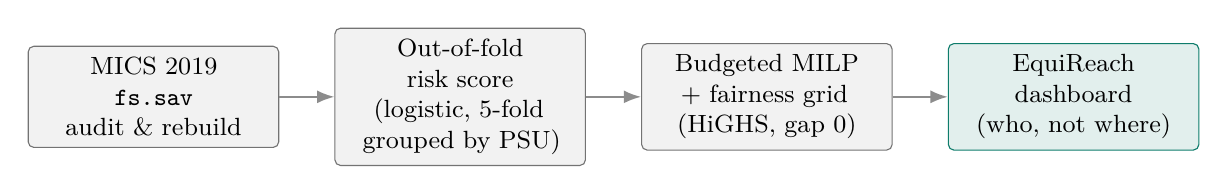
\begin{tikzpicture}[
  node distance=7mm,
  box/.style={draw=black!55, fill=black!5, rounded corners=2pt, align=center,
              text width=2.9cm, minimum height=1.05cm, font=\small, inner sep=4pt},
  live/.style={draw=eqteal, fill=eqteal!12, rounded corners=2pt, align=center,
               text width=2.9cm, minimum height=1.05cm, font=\small, inner sep=4pt},
  arr/.style={-{Latex[length=2.2mm]}, draw=black!45, line width=0.7pt}
]
\node[box] (d) {MICS 2019\\\texttt{fs.sav}\\audit \& rebuild};
\node[box, right=of d] (s) {Out-of-fold\\risk score\\(logistic, 5-fold\\grouped by PSU)};
\node[box, right=of s] (m) {Budgeted MILP\\+ fairness grid\\(HiGHS, gap 0)};
\node[live, right=of m] (w) {EquiReach\\dashboard\\(who, not where)};
\draw[arr] (d) -- (s);
\draw[arr] (s) -- (m);
\draw[arr] (m) -- (w);
\end{tikzpicture}
\caption{The pipeline used in this report. Aggregate microdata are audited and rebuilt, scored out-of-fold, allocated under a fixed budget with optional age and gender floors, and the same selection step is shipped as the EquiReach dashboard.}
\label{fig:pipeline}
\end{figure}

% ── 4. Results ────────────────────────────────────────────────
\section{Results}

\subsection{Baseline and the price of each floor}

The unconstrained risk ranking captures 332 of the 641 observed out-of-school children (51.8\%), but it is badly age-skewed: just 1 selected child is under 13 (0.14\%), while girls make up 29.04\%. The model effectively ignores younger children because risk rises sharply with age here.

Table~\ref{tab:policy} prices the floors. A proportional young floor ($y_{\min}=423$, forcing 57.9\% of the selected set under 13) cuts captured out-of-school children to 219, a loss of 113, for an objective drop of 103.64. A girls-parity floor ($g_{\min}=367$, 50.3\% female) costs only 12 captured children and an objective drop of 12.91. Gender is the cheaper promise because the unconstrained plan already sits near 29\% girls and the risk spread across genders is flatter than across age bands.

\begin{table}[H]
\centering
\renewcommand{\arraystretch}{1.16}
\scriptsize
\resizebox{\textwidth}{!}{%
\begin{tabular}{@{}lrrrrrrrrr@{}}
\toprule
\textbf{Scenario} &
\textbf{Y floor} & \textbf{G floor} & \textbf{Y \%} & \textbf{G \%} &
\textbf{Poorest \%} & \textbf{Objective} & \textbf{Obj drop} &
\textbf{Capt.\ OOS} & \textbf{Interaction} \\
\midrule
Raw risk, no floors      & 0   & 0   & 0.1  & 29.0 & 41.9 & 325.66 & 0.00   & 332 & -- \\
Girls 40\% only          & 0   & 292 & 0.0  & 40.0 & 45.8 & 322.04 & 3.62   & 329 & -- \\
Girls parity only        & 0   & 367 & 0.0  & 50.3 & 45.6 & 312.75 & 12.91  & 320 & -- \\
Young 10\% only          & 73  & 0   & 10.0 & 25.1 & 46.7 & 318.08 & 7.58   & 319 & -- \\
Young 20\% only          & 146 & 0   & 20.0 & 22.9 & 49.7 & 304.27 & 21.39  & 308 & -- \\
Young 33\% only          & 243 & 0   & 33.3 & 24.2 & 52.1 & 280.05 & 45.62  & 291 & -- \\
Young proportional       & 423 & 0   & 57.9 & 23.4 & 56.2 & 222.02 & 103.64 & 219 & -- \\
Young 33\% + Girls 40\%  & 243 & 292 & 33.3 & 40.0 & 55.3 & 276.47 & 49.19  & 278 & $-0.054$ \\
Young 33\% + Girls parity& 243 & 367 & 33.3 & 50.3 & 54.5 & 270.23 & 55.44  & 272 & $-3.095$ \\
Young prop.\ + Girls 40\%& 423 & 292 & 57.9 & 40.0 & 56.4 & 219.23 & 106.44 & 216 & $-0.828$ \\
Young prop.\ + Girls parity & 423 & 367 & 57.9 & 50.3 & 57.1 & 214.85 & 110.81 & 213 & $-5.740$ \\
\bottomrule
\end{tabular}%
}
\caption{Policy scenarios. The objective is the sum of out-of-fold predicted risk scores; observed out-of-school capture is an evaluation metric, not the optimization target. Every row was solved to proven optimality. Interaction is reported only for two-floor rows.}
\label{tab:policy}
\end{table}

\subsection{The two floors are subadditive}

Apply both at their proportional/parity levels ($y_{\min}=423$, $g_{\min}=367$) and the objective drop is 110.81. The separate drops sum to

\begin{equation}
103.64 + 12.91 = 116.55,
\end{equation}

so the interaction is

\begin{equation}
110.81 - 116.55 = -5.74.
\end{equation}

That negative value is subadditivity: the floors behave as complements in cost. Once the plan must admit younger children, the remaining risk pool is reshaped in a way that makes the girls floor cheaper than it would be from the unconstrained baseline. Figure~\ref{fig:fairness} shows this geometrically; in panels C and D the girls floor costs less when the proportional young floor is already active. The poorest share also rises, from 41.9\% to 57.1\%, but that is a side effect of the age and gender floors, not a separate constraint.

\begin{figure}[H]
\centering
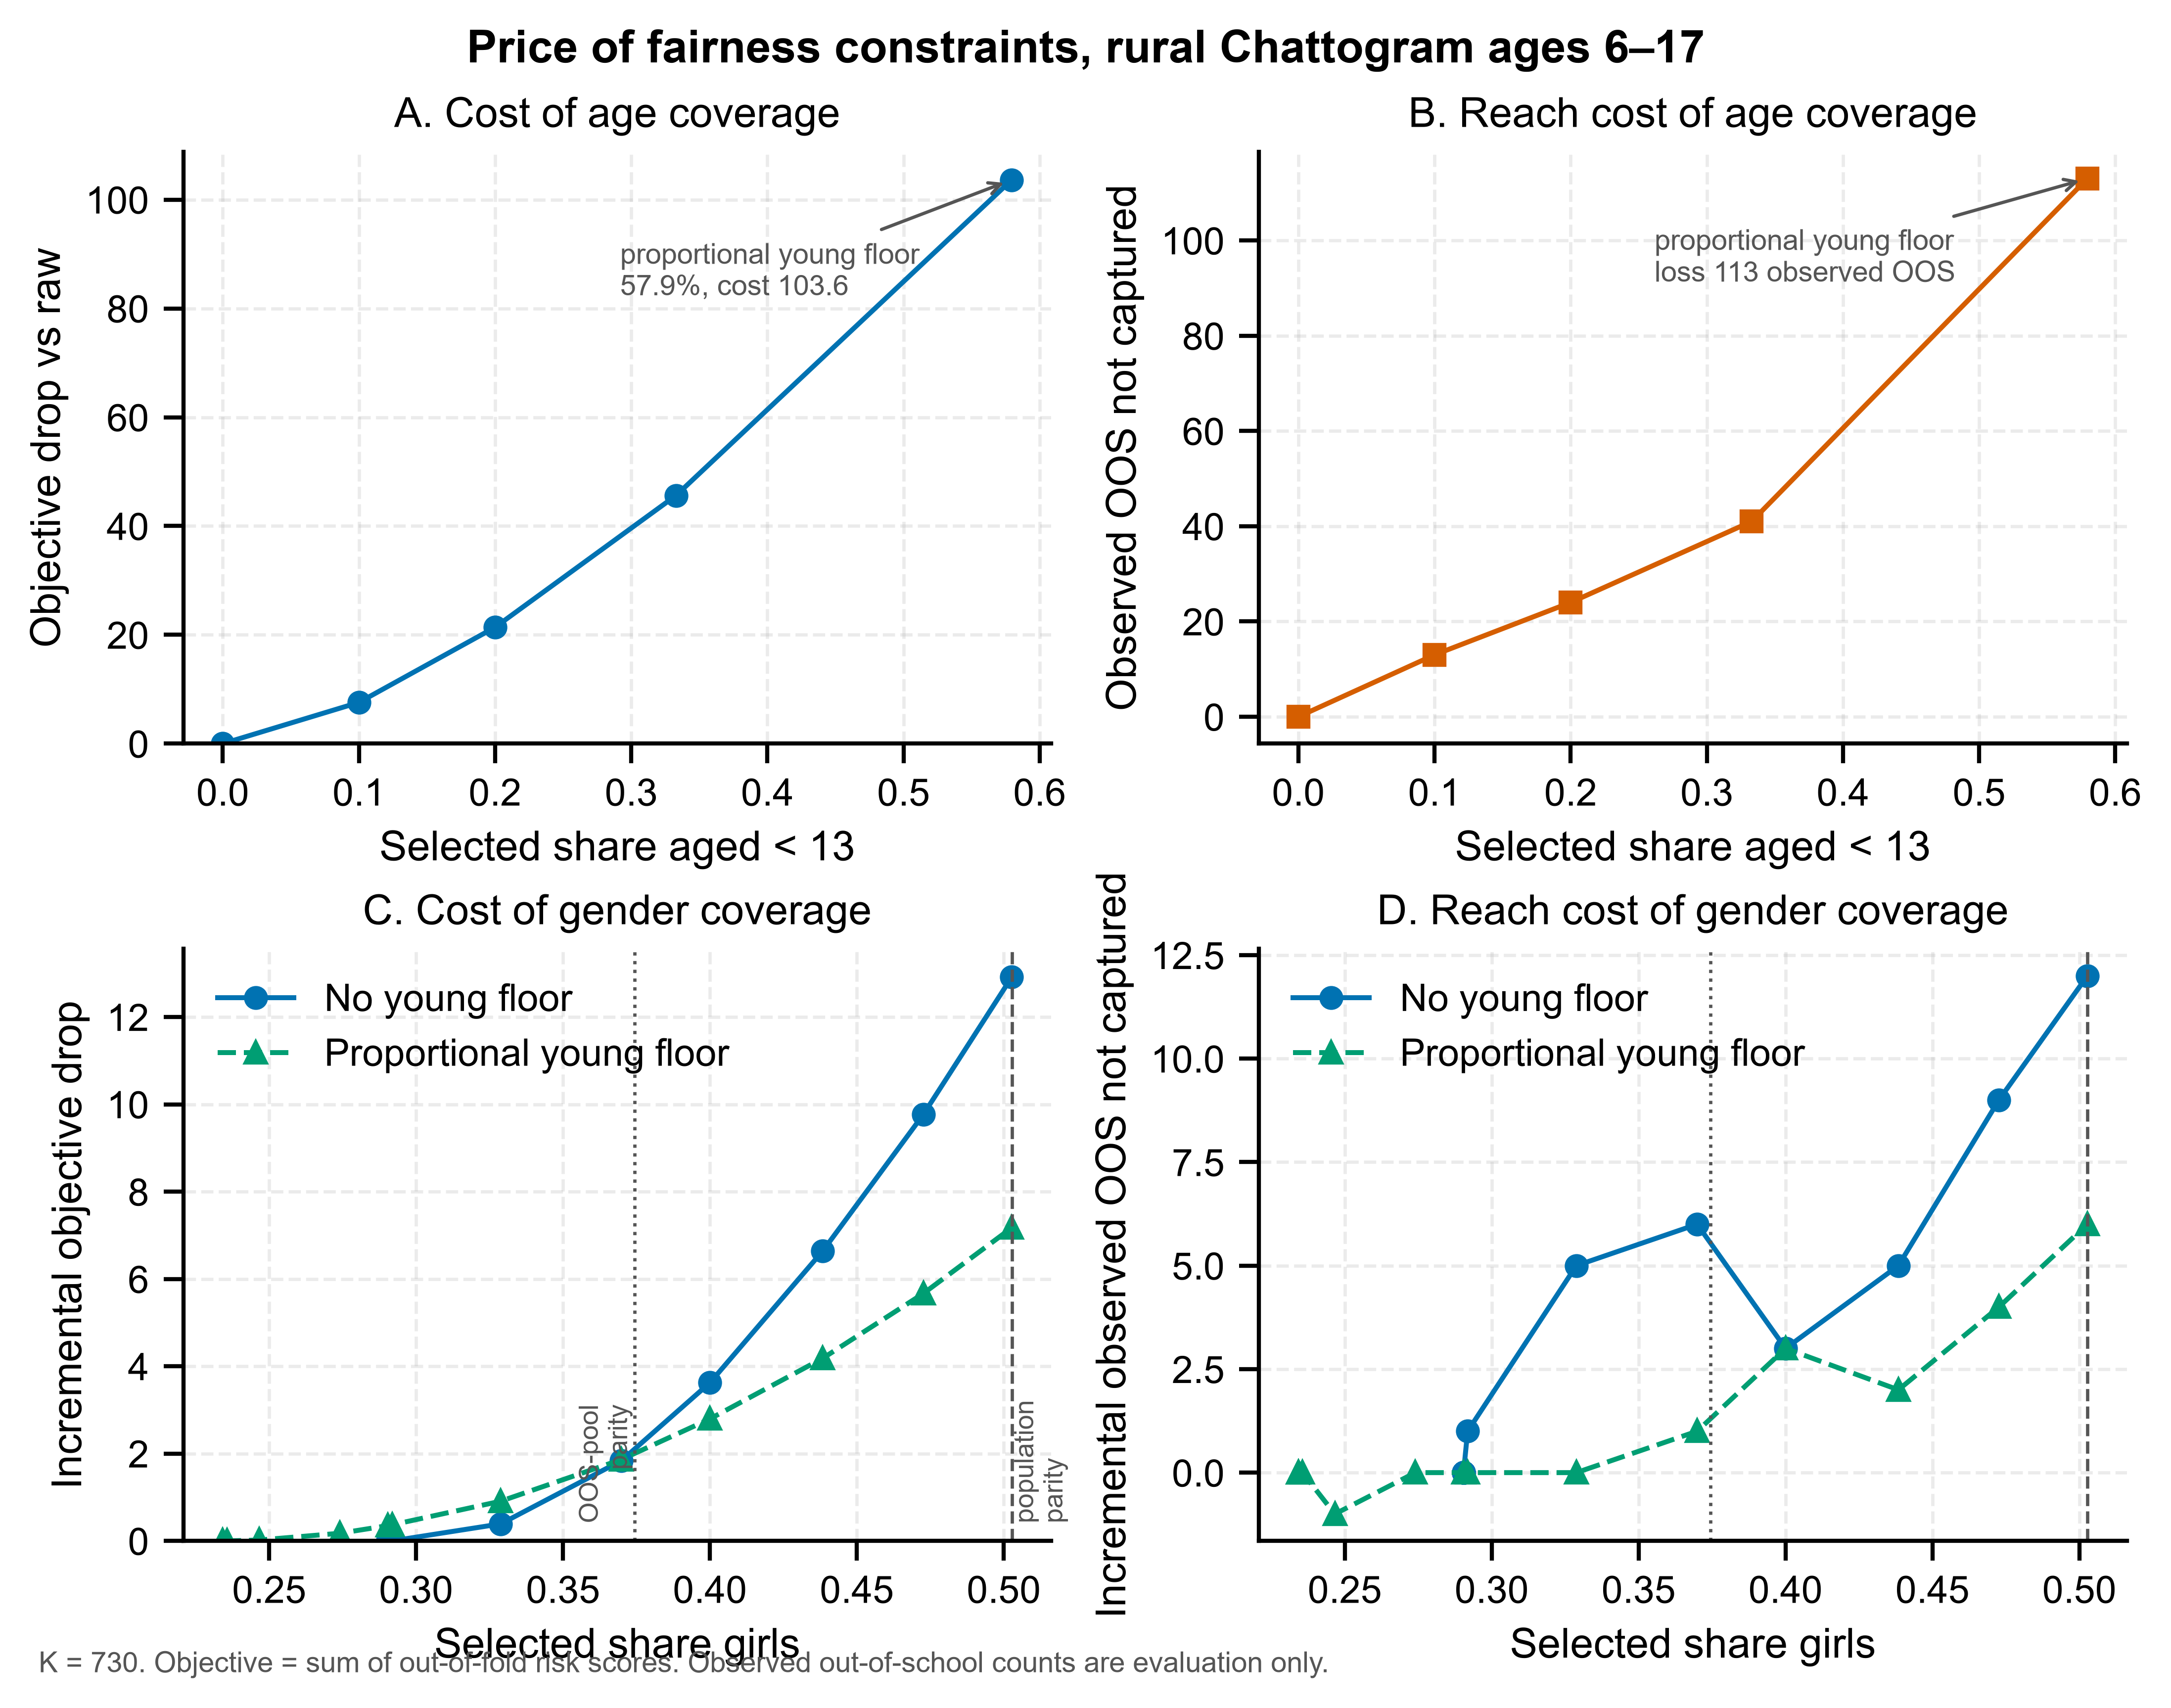
\includegraphics[width=0.97\textwidth]{phase3_fairness_curves_publication.png}
\caption{Price of fairness constraints. Panels A and B price the under-13 floor (objective loss and additional out-of-school children left uncaptured). Panels C and D price the girls floor with and without the proportional under-13 floor. Grey lines mark out-of-school pool parity (37.4\%) and population parity (50.3\%); these are reference points, not constraints. The lower girls-floor cost under the young floor is the subadditivity in Table~\ref{tab:policy}.}
\label{fig:fairness}
\end{figure}

\FloatBarrier

% ── 5. Dashboard ──────────────────────────────────────────────
\section{The EquiReach Dashboard}

I packaged the selection step as EquiReach. It keeps the same Mode A logic: given a budget and optional coverage floors, choose which children receive support. It does not choose where to build centers. The public page is a teaching and preparation tool, not a storage service, and it offers four paths (Table~\ref{tab:paths}).

\begin{table}[H]
\centering
\renewcommand{\arraystretch}{1.25}
\small
\begin{tabular}{@{}p{3.0cm}p{5.4cm}p{3.4cm}p{4.2cm}@{}}
\toprule
\textbf{Path} & \textbf{What it does} & \textbf{Where the data goes} & \textbf{What it returns} \\
\midrule
Guided demo &
Fictional children show the plan, promise checks, and fairness cost. &
Public synthetic API only. &
Selected count, objective, promise status. \\

Own data, prepare file &
Reads CSV, TSV, JSON, or JSON Lines in the browser. &
Stays in the browser. &
\texttt{payload.json} and a local run kit. \\

Own data, calculate here &
Runs one allocation after an explicit consent step. &
One stateless public call; rows not stored. &
Selected \texttt{client\_id} list and summary. \\

Local or private run &
Solves the same model on the user's machine or infrastructure. &
User's device or private system. &
\texttt{result.json} and \texttt{selected\_clients.csv}. \\
\bottomrule
\end{tabular}
\caption{Dashboard paths. Restricted or third-party identifiable records, and very large lists, should use the local download rather than the public server.}
\label{tab:paths}
\end{table}

A real run needs, per child: \texttt{client\_id}, \texttt{priority\_score}, \texttt{weight}, \texttt{age\_band}, \texttt{gender}, \texttt{disability}, \texttt{wealth\_quintile}, and optionally \texttt{need\_flag}. The \texttt{priority\_score} must already be validated; raw attendance labels are not enough on their own, so the user first scores with the project's out-of-fold pipeline or an approved model. The public service is CORS-locked to the project origin and held warm by a scheduled GitHub Actions ping. Those are hosting choices, not model choices.

% ── 6. Reproducibility, privacy, limits ───────────────────────
\section{Reproducibility, Privacy and Limits}

The repository publishes aggregate tables, aggregate curves, figures, code, and documentation only. Raw \texttt{.sav} files and derived child-level CSVs are kept local and never committed; the \texttt{.gitignore} enforces this, and the public tree contains no path under \texttt{data/} and no \texttt{.sav} file. The science rebuilds from the committed scripts and aggregate outputs under \texttt{src/}, \texttt{reports/}, and \texttt{results/}. The \texttt{docs/} folder is maintained directly for the public site and dashboard, and editing it does not affect reproducibility. A Google Colab demo that regenerates the figure and policy table from the aggregate CSVs is published and linked above; this document is the working paper.

Three limits are worth stating plainly.

\begin{itemize}[leftmargin=*, itemsep=3pt]
  \item The risk score is predictive, not causal. It ranks children by estimated out-of-school risk; it does not estimate the effect of support.
  \item The MICS children's file has no household coordinates, school or upazila identifiers, travel distances, construction costs, or center capacities. The dashboard answers \emph{who}, not \emph{where}.
  \item The weighted out-of-school rate is provisional because the weight definition was corrected late in the audit; \texttt{fsweight} is primary and \texttt{fshweight} is a sensitivity check.
\end{itemize}

AI tools helped scaffold the dashboard and debug front-end code, and helped draft parts of this text. Every methodological decision, data check, number, and final wording was reviewed and approved by me, and a dated step-by-step record of the AI-assisted work is kept in the repository's AI-use log.

% ── 7. Conclusion ─────────────────────────────────────────────
\section{Conclusion}

Pure risk targeting reaches many out-of-school adolescents while nearly excluding younger children, and explicit coverage floors carry a real price in reach. That price is not simply additive across groups. In this rural Chattogram sample, age coverage is expensive, gender parity is comparatively cheap, and the two floors are subadditive at the proportional corner, so a programme that wants both pays less than the separate costs suggest. The dashboard turns the same selection model into something a practitioner can test on fictional data or prepare for local use with their own file, while keeping restricted records off the public server. Extending the work to \emph{where} support should be located would require collecting distance, cost, and capacity data that the survey does not contain, which is the natural next phase rather than a claim this report makes.

% ── References ────────────────────────────────────────────────
\begin{thebibliography}{9}
\setlength{\itemsep}{4pt}

\bibitem{mics2019}
UNICEF and Bangladesh Bureau of Statistics.
\textit{Bangladesh Multiple Indicator Cluster Survey 2019}.
Dhaka, Bangladesh, 2020.

\bibitem{scipy}
Virtanen, P., Gommers, R., Oliphant, T.~E., et al.
\textit{SciPy 1.0: Fundamental Algorithms for Scientific Computing in Python}.
Nature Methods, 17, 261--272, 2020.

\bibitem{highs}
Huangfu, Q., and Sanderson, J.~J.
\textit{Parallelizing the dual revised simplex method}.
Mathematical Programming Computation, 10(1), 119--142, 2018.

\end{thebibliography}

\end{document}